\chapter{Arquitectura de Referencia del Browser}
\label{chap4:ArqRefBrowser}

La arquitectura de referencia a construir en este trabajo tiene como objetivo catalizar el entendimiento de la estrecha relación que existe entre el \cite{Web Browser} y los sistemas que serían construídos sobre la Internet. En vista a la poca, casi nula, documentación de la creación de Arquitecturas de Referencias del Navegador Web, la necesidad de hacer una AR para entender cómo la arquitectura de este sistema puede relacionarse con el futuro desarrollo de otros sistemas, llega a ser imperante. Al considerar al Web browser como un \textit{concern} en el desarrollo de SoftWare puede ser una buena estrategia para evitar una gran perdida monetaria u organizacional. Se sabe que el Browser es un pieza de Software que ha sufrido varios cambios desde la década de los 90, por lo tanto entre los desarrolladores de ésta herramienta ya existen conveniones de qué elementos funcionan mejor. Por consiguiente, no es de extrañar que diferentes browsers estén construidos de formas muy similares, y en consecuencia puedan ser conceptualizados en una Arquitectura de Referencia que manifeste los componentes, mecanismos de comunicación y funciones de esta pieza de Software.

En este capítulo se presenta una Arquitectura de Referencia (AR) desarrollada principalmente a partir de la abstracción de las propuestas existentes hoy em día como: Google Chrome/Chromium, Internet Explorer y Firefox; nos basaremos en información del año 2014 hacia atrás. Primero se identificarán y analizarán los stakeholders, se identificarán los casos de uso relacionados a uno de estos stakeholders y se dará una descripción breve. Luego se presentarán patrones que formarán parte de nuestra AR. Éstos patrones serán descritos utilizando un template POSA \cite{buschman1996system} y notación UML para precisar cómo los componentes de la AR se relacionan.


\section{Casos de Uso del Browser}
	\subsection{Stakeholders (actores) y Concerns de estos}
	Se es necesario encontrar los actores (definido por sus roles) que participan en el uso y operación del Navegador, estos son:
		\subsubsection{Usuario Consumidor (UC)}
		Este es el principal stakeholder, pues de él depende que se realice el inicio de una petición para buscar una página web, recurso o servicio. Sin éste la utilidad del Web Browser es nula. El stakeholder al mismo tiempo podría ser una entidad no humana, como un plugin, extensión o instancia de una página web, que requiere hacer peticiones por medio de las interfaces del navegador, pero que al fin y al cabo cumplen con los deseo del usuario del host de mostrar el contenido.

		\subsubsection{Sistema Operativo (SO)}
		Crea el o los procesos necesarios para iniciar el Navegador, además de entregar un ambiente al Browser para que éste pueda funcionar adecuadamente. En base al enfoque de este estudio, ésta identidad se encarga de aplicar políticas de seguridad sobre el Browser cuando se necesiten realizar operaciones o el navegador desee crear nuevos procesos.

		\subsubsection{Proveedor de Servicios (PS)}
		Este puede ser un: Web Server, Web Aplicación, Servicio de actualización del Browser, etc. Su interacción con el Browser se limita a entregar contenido a éste, no a usarlo.

	\subsection{Casos de Uso}
	\subsubsection{Casos de Uso para Usuario Consumidor}
		El usuario consumidor es el más importante stakeholder del web browser, pues sin él no habría razón para la existencia del browser; un servidor tampoco existiría dado el mismo principio. Bajo ésta entidad es que suceden la mayoría de los casos de uso del sistema al que realizaremos su AR. Al encontrar los casos de uso de éste stakeholder veremos los concerns de éste, lo que nos permitirá entender las necesidades de seguridad para proteger al navegador.
			\begin{enumerate}
				\item Usar datos privados de usuario (opcional): dependiendo del navegador, se podría indicar al usuario si quiere usar una cuenta externa o interna para acceder a información propia de usuario consumidor y mejor así la experiencia de usuario.

				\item Realizar Petición/Request: El caso de uso más importante de éste sistema y en la que se basa la arquitectura cliente/servidor. Esta acción considera encontrar el recurso bajo la URI dada y la consecuente descarga del recurso. La descarga no es siempre necesaria, pues existe lo que se conoce como una peticiíon \textit{preflight} donde solo se envía una petición para saber si es seguro realizar una petición/request. Entonces como una consideración a este caso de uso es que una petición/request no siempre conlleva una respuesta/response, por lo que hemos condensado estas dos (request/response) en un solo caso de uso. 

				\item Descargar recurso: Este caso de uso está incluído dentro de Petición/Request, pues para conseguir una página web es necesario la descarga del recurso.

				\item Solicitar intervención: exiten oportunidades en que la realización de una petición/request conllevará a que el Browser pida permiso al UC para realizar otras acciones, ejemplo: instalar un plug-in, extensión, descargar un contenido que no se puede evaluar su seguridad. En los casos anteriores, una ventana de la interfaz gráfica pedira explícitamente la intervención del usuario para tomar una decisión.

			\end{enumerate}

		Existen muchos más casos de uso relativos al stakeholder tomado, pero para este trabajo bastarán con los propuestos. Una vez que sabemos los roles involucrados y la forma en que interactuan con el sistema, será posible encontrar las amenazas contra el browser.

		\subsubsection{Casos de Uso para el Sistema Operativo}
			\begin{enumerate}
				\item Operación CRUD en host: Acción realizada cuando el Browser obtiene una solicitud explícita o no (automática), del usuario para realizar acciones que involucren permitir un acceso desde el sistema operativo como: leer, escribir o modificar/eliminar algún recurso del host.

				\item Recibir solicitud: En un browser es normal la comunicación entre los procesos que lo componen y el Sistema operativo por medio de un canal de comunicación, ejemplo de esto es cuando un plug-in se comunica con el proceso encargado de mostrar por pantalla lo que se hace en él.
			\end{enumerate}

		\subsubsection{Casos de Uso para el Proveedor de Servicios}

			\begin{enumerate}
				\item Recibir Petición/Request: El PS siempre está escuchando en sus puertos habilitados a posibles peticiones de sus clientes. Una petición es recibida en un formato que el PS debe saber interpretar y en consecuencia realizar las acciones correspondientes que el cliente le pide. Por cada solicitud del cliente, en este caso el Web Browser, habrá una respuesta/response por parte del PS. Este caso de uso no se ejecuta, si dentro del header de uno de los paquetes está indicado que la petición fue hecha en modo \textit{preflight}.

				\item Operación CRUD: alguna petición podría terminar por realizar un cambio en el PS dado por alguna operación CRUD. Éstas opciones son la voluntad del usuario en el host, y que son transmitidas y realizadas indirectamente por el Web Browser.
			\end{enumerate}

		Los casos de Uso descritos anteriormente se pueden divisar en la Figura \ref{fig:CUBrowser}

	    \begin{figure}[h]
	        \centering
	        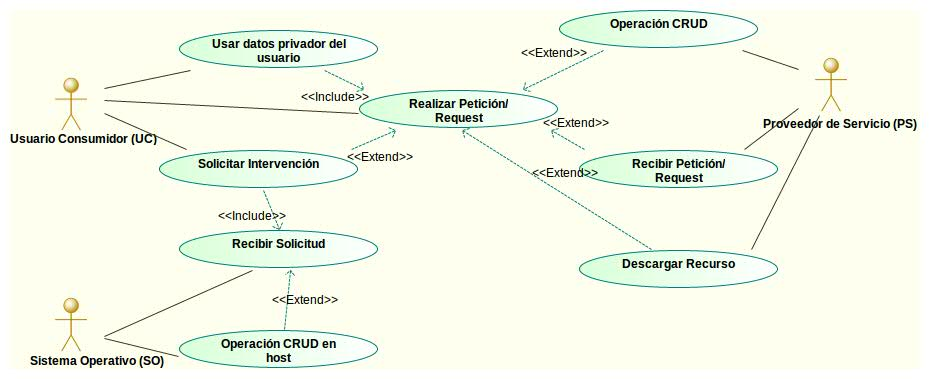
\includegraphics[scale=0.45]{figures/CUBrowser.jpg}
	        \caption{Diagrama de Caso de Uso del Web Browser}
	        \label{fig:CUBrowser}
	    \end{figure}



\section{Patrón Broker/Frame/Browser Engine/Process (BP)}
\label{chap4:BrokerPatt}
\subsection*{Intent}
El patrón Broker/Frame/Browser Engine/Process o BP 


\subsection*{Ejemplo}

\subsection*{Contexto}

\subsection*{Solución}

\subsection*{Estructura}

\subsection*{Dinámica}

\subsection*{Consecuencias}

\subsection*{Ejemplo Resuelto}

\subsection*{Usos Comúnes}

\subsection*{Patrones Asociados}

\newpage

\section{Patrón Rendering Engine (RE)}
\label{chap4:REPatt}
\subsection*{Intent}
El patrón Rendering Engine o RE representa a todos los componentes necesarios para realizar el parsing y layout de HTML y XML, interpretación de javascript, construcción del DOM y las interfaces limitadas para la comunicación entre procesos con el BP, para el posterior display de la información por pantalla usando Sistema Operativo (SO).


\subsection*{Ejemplo}

\subsection*{Contexto}

\subsection*{Solución}

\subsection*{Estructura}

\subsection*{Dinámica}

\subsection*{Consecuencias}

\subsection*{Ejemplo Resuelto}

\subsection*{Usos Comúnes}

\subsection*{Patrones Asociados}

\newpage

\section{Patrón User Interface}
\label{chap4:UIPatt}
\subsection*{Intent}

\subsection*{Ejemplo}

\subsection*{Contexto}

\subsection*{Solución}

\subsection*{Estructura}

\subsection*{Dinámica}

\subsection*{Consecuencias}

\subsection*{Ejemplo Resuelto}

\subsection*{Usos Comúnes}

\subsection*{Patrones Asociados}

\newpage

\section{Patrón Plugin}
\label{chap4:PluginPatt}
\subsection*{Intent}

\subsection*{Ejemplo}

\subsection*{Contexto}

\subsection*{Solución}

\subsection*{Estructura}

\subsection*{Dinámica}

\subsection*{Consecuencias}

\subsection*{Ejemplo Resuelto}

\subsection*{Usos Comúnes}

\subsection*{Patrones Asociados}

